%%%%%%%%%%%%%%%%%%%%%%%%%%%%%%%%%%%%%%%%%%%%%%%%%%%%%%%%%%%%%%%%%%%%%%%%%%%%%%%%

\documentclass[letterpaper, 10 pt, conference]{ieeeconf}
\setlength{\parskip}{\baselineskip}
% \setlength{\parindent}{0pt}


                                                          % Comment this line out
                                                          % if you need a4paper
%\documentclass[a4paper, 10pt, conference]{ieeeconf}      % Use this line for a4
                                                          % paper

\IEEEoverridecommandlockouts                              % This command is only
                                                          % needed if you want to
                                                          % use the \thanks command

\overrideIEEEmargins
% See the \addtolength command later in the file to balance the column lengths
% on the last page of the document



% The following packages can be found on http:\\www.ctan.org
\usepackage{graphicx} % for pdf, bitmapped graphics files
\graphicspath{{./images/}}
%\usepackage{epsfig} % for postscript graphics files
%\usepackage{mathptmx} % assumes new font selection scheme installed
%\usepackage{times} % assumes new font selection scheme installed
%\usepackage{amsmath} % assumes amsmath package installed
%\usepackage{amssymb}  % assumes amsmath package installed
\usepackage{tabulary}
\usepackage{array}

\title{\LARGE \bf
Timbre Music Recommendation System
}

\author{Chase Ehlert$^{1}$% <-this % stops a space
\thanks{*This work was supported by Oakland University}% <-this % stops a space
\thanks{$^{2}$Chase Ehlert is a graduate student in the college of Engineering and Computer Science, at Oakland University, 2200 Squirrel Rd, Rochester, MI 48309, USA
        {\tt\small cwehlert at oakland.edu}}%
}

\begin{document}

\maketitle
\thispagestyle{empty}
\pagestyle{empty}

%%%%%%%%%%%%%%%%%%%%%%%%%%%%%%%%%%%%%%%%%%%%%%%%%%%%%%%%%%%%%%%%%%%%%%%%%%%%%%%%

\begin{abstract}
Developing an efficient and successful music recommendation system could levy a large user base and help to promote a music based application. If a new recommendation system were created from evaluating the timbre values of music, it could help to launch a unique and successful application. This paper describes one method for developing a music recommendation system not used today in an effort to break ground in an undiscovered area. The results gathered from testing the recommendation system developed, show that it will recommend music similar to what the user has chosen as favorited songs at close to a $50\%$ liked rate.

\end{abstract}

%%%%%%%%%%%%%%%%%%%%%%%%%%%%%%%%%%%%%%%%%%%%%%%%%%%%%%%%%%%%%%%%%%%%%%%%%%%%%%%%

\section{INTRODUCTION}
In today’s world of social networking and smartphone technology, developing a popular app can be extremely beneficial. Music based apps are also popular leveraging how the majority of society use smartphone applications every day in their lives. A favorite feature of these music apps is to listen to “radio” stations in which the app will generate music similar to what the user already likes. The timbre features of music can provide a unique way of classifying different genres of music to find commonaliities between them. The remainder of this paper is organized as follows. Section 2 reviews the research in the field of developing and testing different music recommendation systems. Section 3 covers my approach to developing a timbre based music recommendation system and what timbre is in relation to music. Section 5 describes the setup of my recommendation system and how it was tested. Section 6 reviews the results gathered from the recommendation system developed and outlines the reasoning behind altering the initial system. Section 7 concludes the paper.

%%%%%%%%%%%%%%%%%%%%%%%%%%%%%%%%%%%%%%%%%%%%%%%%%%%%%%%%%%%%%%%%%%%%%%%%%%%%%%%%%%%%%%%%%%

\section{RELATED WORK}
% It describes the existing work related to the work in the report. It should not be more than one page. Position our work in current research (length depends on number of papers)
In Patel and Wadhvani’s paper titled A Comparative Study of Music Recommendation Systems they examine the performance of two different types of music recommendation systems, a Preference-linked and Positive Graph-based algorithm (PPGB) and an Incremental Regression Tree (IRT) \cite{two}. The PPGB works by building two graphs based on a user’s listening record and ratings they’ve given to songs. This algorithm will then combine both graphs to form the recommendation results. Challenges that are faced with this model are a cold start issue and a potential of lack of ratings from the user. The cold start problem could come about by the difficulty of recommending music to a user that hasn’t listened to a lot of music. The IRT is a lightweight data structure meant for the limiting space and power of smartphones. It is a decision tree that blends incremental modeling and collects three different types of data related to the songs that have been listened to. The different types of data that are collected are the listening contexts, the audio features of the song, and the rating given by the user for the songs. This model has a quality feature of having a clear separation of nodes for each Music Record Cluster but may also be subject to the lack of ratings from a user problem.

Wu’s paper titled Music Personalized Recommendation System Based on Hybrid Filtration investigates the performance of a model based on recommending music listened to by other users with similar tastes \cite{three}. The model developed by Wu first uses collaborative filtering to divide users of the app into groups of different interests and evaluating said users and groups of users similarly. The model basis of examining music is to look at what Wu describes as the Music Gene. This gene is made up of two groups of classifiers, internal-genes and social-genes. The internal-genes are traits of music such as: lyric, melody, rhythm, and speed. The social-genes are traits of music such as: the name of the music, composer, singer, and style. Wu’s experiment tests the performance of three different recommendation systems, collaborative filtering, music gene, and a combination of both. Wu discovered that the system using a combination of both collaborative filtering and the music gene garnered the best results for recommending music that user’s liked.

In Girsang, Wibowow, and Edwin’s paper titled Song Recommendation System Using Collaborative Filtering Methods they investigate a model also based on collaborative filtering \cite{four}. This model will weigh the similarities between users and will be computationally light compared to content-based approaches. The group carried out their experiments by taking a variable amount of neighbors to a specific user and then selecting the neighbors by the highest rated song listen count. They then compare the neighbor’s by using the Pearson’s Correlation function and recommending the neighbor with the highest score. The results for their experiment showed that the model had an accuracy of greater than $70\%$ liked songs by $95\%$ of the users that participated in the experiment.

In Rosa, Rodriguez, and Bressan’s paper titled Music recommendation system based on user's sentiments extracted from social networks they investigate how the influence of social media can affect what music someone might want to listen to \cite{five}. Their model uses a word dictionary called Sentimeter-Br2 to evaluate the words and phrases posted from a user of the recommendation system. This dictionary will assign a positive or negative association with the post, the categories of the associations are: happiness, sadness, anger, romance, and gentleness. The experiment performed by the group collects phrases from the users every hour over the course of three weeks. If the user does not post anything for the system to collect then the system will recommend music based on the music preference given by the user. What the experiment showed was that negative sentiments were found to change on a regular basis, the social media influenced system had a higher success rate than the music recommended by the music preference suggested by the user. The experiment also showed that the emotional state of someone can influence their desired taste in what kind of music they’d like to listen to.
In Bai and Kawagoe’s paper titled Background Music Recommendation System

Based on User's Heart Rate and Elapsed Time develops a model based on the user’s psychosomatic condition \cite{six}. In their paper Bai and Kawagoe test how two different recommendation systems based on the user’s heart rate perform with this influence in recommending the user music. The first model called BMR-HR uses the user’s heart rate to recommend music. The second model BMR-HNE uses a combination of the user’s heart rate, music preference, and activity time to recommend music. A third model is used which will recommend random music from a selection of music. The models were tested by the users rating the recommended songs on a 1 - 5 scale and an appropriate rate which was measured by the number of liked songs against the total number of songs. After testing the performance of all three models, BMR-HR model was the most favored, the random selection was the least favored, and both BMR-HR and BMR-HNE appropriate rates were discovered to not be practical.

%%%%%%%%%%%%%%%%%%%%%%%%%%%%%%%%%%%%%%%%%%%%%%%%%%%%%%%%%%%%%%%%%%%%%%%%%%%%%%%%%%%%%%%%%%

\section{APPROACH}
% Describe the proposed solution to address the problem. This is the most important section. Be concrete and clear. Use of diagrams help organize the approach and improve understanding. Every diagram must be explained in text before the diagram
The method of classifying music based on it’s timbre values is an unexplored area of research. Timbre is a method of classifying the different sounds of music. It can be described as the character of a musical note that can differentiate between different types of voices or musical instruments \cite{one}. The dataset used to develop and test both of the recommendation models detailed in this paper includes two sets of timbre values. The first set contains the average of each of the twelve timbre features measured throughout a song. The second set contains the variance of the same twelve timbre features. A combination of these 24 timbre values are used as the features for clustering the songs used in the dataset.

%%%%%%%%%%%%%%%%%%%%%%%%%%%%%%%%%%%%%%%%%%%%%%%%%%%%%%%%%%%%%%%%%%%%%%%%%%%%%%%%%%%%%%

\section{EXPERIMENTAL SETUP}
The first timbre based recommendation model created uses music taken from every genre in the dataset to use for clustering and will be referred to as model X. It begins by finding the indexes of the liked songs submitted by a user to reference in the KMeans clustered dataset later on. This is done to find out later which clusters the liked songs have ended up in, as with how I handle the dataset that will be the only way to follow the liked songs. After collecting the indexes of user-liked songs the model will then join them in a dataframe with 100 other songs made up of ten songs for ten different genres. These songs were not in the dataset of songs the user had a choice to pick from. This dataframe of songs is then clustered by KMeans clustering to a factor of ten clusters. The aim with clustering the songs in this manner is to evaluate how effective measuring music by its associated timbre features will cluster separately. Then after the clusters have been created the model will collect the cluster labels for the clusters that contain the liked songs. Next the model will collect five songs to recommend to the user by removing the liked songs from the dataframe and collecting every song in each of the clusters collected. The model will then pick at random from this list to recommend songs to the user, I tested this model out on three volunteers. This method of recommending songs did not prove to be useful, which will be detailed later in the results section. I altered the model in hopes to increase its effectiveness at recommending music to users that they would like to listen to, this model will be referred to as model Y. This alteration is focused on including only the genres of music the user liked to use for clustering. The changes to the model include evaluating what genre the songs liked by the user belong to. Then the model will collect all music that is tagged with this genre in the dataset. This collection of music is then combined with the liked songs and KMeans clustered by four different factors: 10, 20, 40, and 80. After the songs have been clustered the model will then collect the cluster labels of each cluster the liked songs were placed in and a song is chosen at random from these clusters to recommend.

%%%%%%%%%%%%%%%%%%%%%%%%%%%%%%%%%%%%%%%%%%%%%%%%%%%%%%%%%%%%%%%%%%%%%%%%%%%%%%%%%%%%%%

\section{RESULTS}
Three volunteers were used to test both music recommendation models created. To test the models the users chose five songs they liked from the initial dataset and five songs were then recommended based off of these seeds. The three users (to be referred to as A, B, and C) provided the results for the effectiveness of model X in Figure 1. After determining that model X was not at least $50\%$ effective at recommending songs the user will like, the model was then altered in an effort to increase the effectiveness of a timbre based recommendation system. The same seeds used for model X from the three users were then used in model Y to generate the results shown in Figure 2.

\begin{figure}[h]
        \centering
        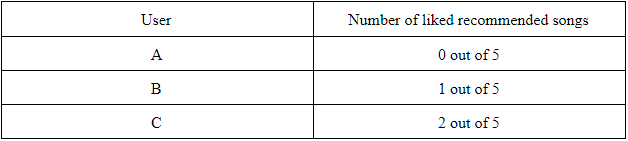
\includegraphics[width=8.6cm]{modelX.png}
        \caption{Model X Results}
        \label{fig:ecnoc}
\end{figure}

\begin{figure}[h]
        \centering
        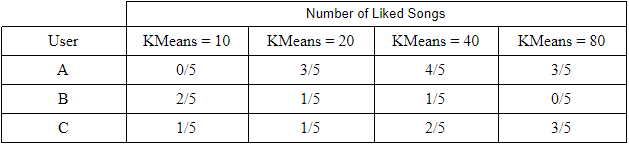
\includegraphics[width=8.6cm]{modelY.png}
        \caption{Model Y Results}
        \label{fig:ecnot}
\end{figure}

The results from using model Y with a KMeans equal to ten averaged with a user liked rate of $20\%$, KMeans equal to 20 averaged with a user liked rate of about $33\%$, KMeans equal to 40 averaged with a user liked rate of about $47\%$, and a KMeans equal to 80 averaged with a user liked rate of $40\%$. The highest effectiveness with model Y given by the tests performed was the version of the model using a KMeans of 40.

Future Work: Model Y did prove to increase the likelihood of a user liking the recommended songs given but it still did not break an average of a $50\%$ like rate among the users tested. I would not define this as successful unfortunately. With model Y leveraging the best results a different approach could be applied to see if a higher success rate can be achieved. Instead of using both sets of average and variance timbre values, the sets could be tested individually to see if it helps. If that theory does not increase the like rate of the recommended songs, then maybe recommending music based on timbre values does not yield the best solution.

%%%%%%%%%%%%%%%%%%%%%%%%%%%%%%%%%%%%%%%%%%%%%%%%%%%%%%%%%%%%%%%%%%%%%%%%%%%%%%%%%%%%%%%%

\section{CONCLUSIONS}
% Describe lessons learned and remaining work. It should not be more than half page.
% TODO - Write after completing results section

Model Y did prove to increase the likelihood of a user liking the recommended songs given but it still did not break an average of a $50\%$ like rate among the users tested. I would not define this as successful unfortunately. With model Y leveraging the best results a different approach could be applied to see if a higher success rate can be achieved. Instead of using both sets of average and variance timbre values, the sets could be tested individually to see if it helps. If that theory does not increase the like rate of the recommended songs, then maybe recommending music based on timbre values does not yield the best solution.
%%%%%%%%%%%%%%%%%%%%%%%%%%%%%%%%%%%%%%%%%%%%%%%%%%%%%%%%%%%%%%%%%%%%%%%%%%%%%%%%%%%%%%%%

\addtolength{\textheight}{-12cm}   % This command serves to balance the column lengths
                                  % on the last page of the document manually. It shortens
                                  % the textheight of the last page by a suitable amount.
                                  % This command does not take effect until the next page
                                  % so it should come on the page before the last. Make
                                  % sure that you do not shorten the textheight too much.

%%%%%%%%%%%%%%%%%%%%%%%%%%%%%%%%%%%%%%%%%%%%%%%%%%%%%%%%%%%%%%%%%%%%%%%%%%%%%%%%

% \section*{APPENDIX}
% Appendixes should appear before the acknowledgment.
% Optional

%%%%%%%%%%%%%%%%%%%%%%%%%%%%%%%%%%%%%%%%%%%%%%%%%%%%%%%%%%%%%%%%%%%%%%%%%%%%%%%%

% \section*{ACKNOWLEDGMENT}
% Put sponsor acknowledgments in the unnumbered footnote on the first page.
% Optional

%%%%%%%%%%%%%%%%%%%%%%%%%%%%%%%%%%%%%%%%%%%%%%%%%%%%%%%%%%%%%%%%%%%%%%%%%%%%%

\begin{thebibliography}{99}

\bibitem{one} We Know Music... (n.d.). Retrieved from http://the.echonest.com/

\bibitem{two} Patel, A., \& Wadhvani, R. (2018). A Comparative Study of Music Recommendation Systems. 2018 IEEE International Students Conference on Electrical, Electronics and Computer Science (SCEECS). doi: 10.1109/sceecs.2018.8546852.

\bibitem{three} Wu, D. (2019). Music Personalized Recommendation System Based on Hybrid Filtration. 2019 International Conference on Intelligent Transportation, Big Data \& Smart City (ICITBS). doi: 10.1109/icitbs.2019.00112

\bibitem{four} Girsang, A. S., Wibowo, A., \& Edwin. (2019). Song Recommendation System Using Collaborative Filtering Methods. Proceedings of the 2019 The 3rd International Conference on Digital Technology in Education. doi: 10.1145/3369199.3369233

\bibitem{five} Rosa, R. L., Rodriguez, D. Z., \& Bressan, G. (2015). Music recommendation system based on users sentiments extracted from social networks. 2015 IEEE International Conference on Consumer Electronics (ICCE). doi: 10.1109/icce.2015.7066455

\bibitem{six} Bai, K., \& Kawagoe, K. (2018). Background Music Recommendation System Based on Users Heart Rate and Elapsed Time. Proceedings of the 2018 10th International Conference on Computer and Automation Engineering - ICCAE 2018. doi: 10.1145/3192975.3193013

\end{thebibliography}




\end{document}
